La búsqueda binaria es un algoritmo en que se utilizan operaciones lógicas como AND y OR con el fin de encontrar documentos que contienen los términos solicitados en la consulta, asumiendo que ello indica que son relevantes para dicha necesidad de información. Para llevar a cabo la búsqueda de manera eficiente, se crea una matriz binaria indicando los términos que contiene cada documento, dando a la técnica el nombre de \textit{búsqueda binaria}. A continuación, se explica detalladamente el proceso que sigue la técnica.

\subsubsection{Funcionamiento de BS}
Una vez se conoce de cada documento los términos que contiene y su frecuencia, se procede a construir la matriz binaria. Las filas de esta matriz corresponden a los documentos que se consideran en la búsqueda y las filas corresponden a los términos existentes en el diccionario. Siendo así, los registros de cada columna que corresponden a uno indican que ese término existe en el documento indicado por la columna. Cabe resaltar que la frecuencia no es considerada en esta técnica. En la figura \ref{fig:b_matrix} se muestra un ejemplo de cómo se vería una matriz binaria.\\

\begin{figure}[H]
    \centering
    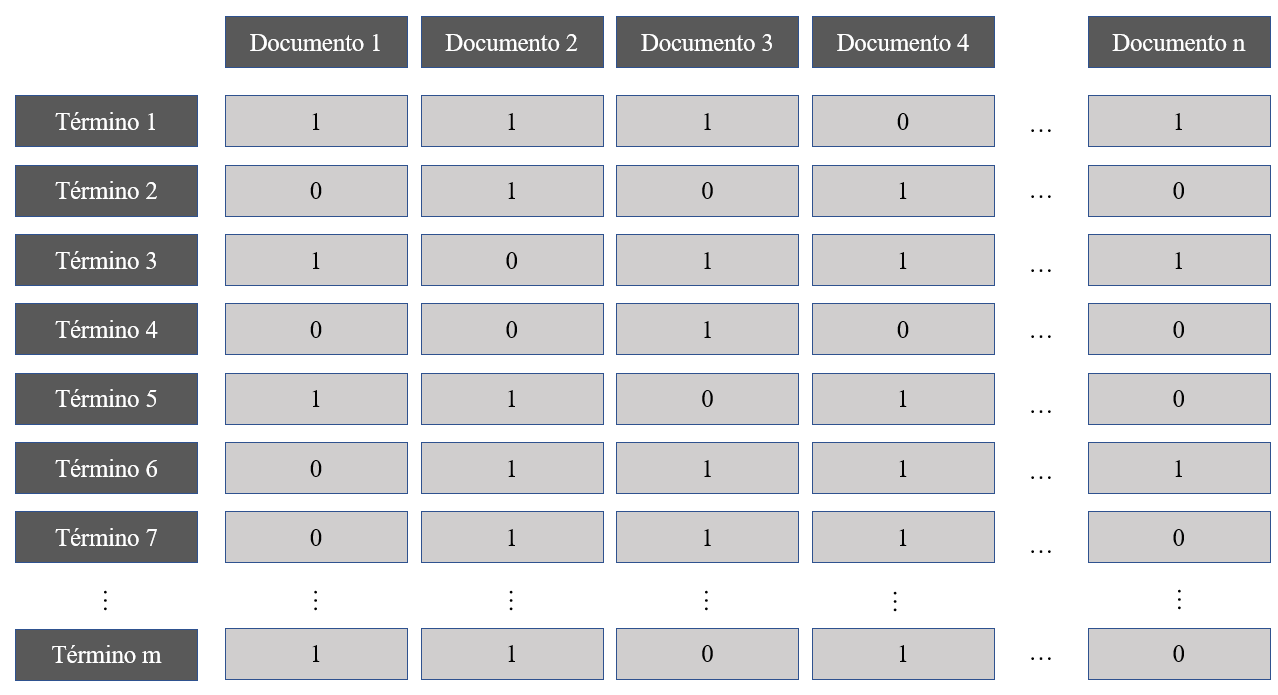
\includegraphics[scale=0.5]{doc/images/BS/b_matrix.PNG}
    \caption{Matriz binaria ejemplo}
    \label{fig:b_matrix}
\end{figure}

Tras recibir la consulta (palabras claves que caracterizan la necesidad de información) se procede a construir un vector del tamaño del vocabulario que indica, al igual que la matriz, qué términos incluye la consulta, generando así un vector binario disperso. En la figura \ref{fig:b_query} se muestra cómo sería el vector de la consulta.\\

\begin{figure}[]
    \centering
    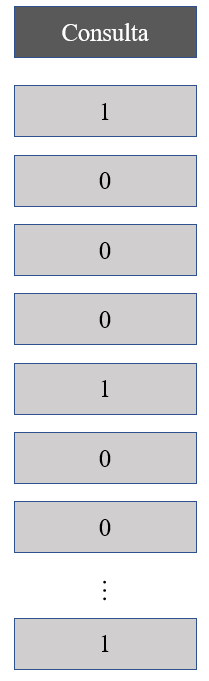
\includegraphics[scale = 0.5]{doc/images/BS/b_query.PNG}
    \caption{Vector binario de la consulta}
    \label{fig:b_query}
\end{figure}

En el caso específico del \textit{dataset} trabajado la matriz tiene dimensión de 17.365 filas, 331 columnas, dado que se tiene un vocabulario de 17.365 términos.\\

Con el fin de almacenar de manera eficiente una matriz de tamaño (5'747.815) se procede a utilizar el tipo de dato que menor espacio de memoria ocupa. Al momento de crear la matriz se indica el tipo de dato a utilizar, el cual corresponde a \url{numpy.bool\_}. Para guardar y abrir la matriz se utilizan las funciones estándar de numpy (\url{load} y \url{save}).\\

Ahora bien, una vez se tiene el vector que representa la consulta y la matriz que almacena toda la información de términos por documento, se utiliza una operación lógica que permita seleccionar los documentos que contienen uno o todos los términos consultados. En el primer caso se utiliza la operación lógica OR, lo cual indica que se extraerán los documentos que tienen al menos uno de los términos buscados; en caso contrario, se utiliza AND para obtener los documentos que tienen todos y cada uno de los términos buscados.\\

Como es de esperarse es poco común que un documento contenga exactamente todos los términos al igual que es muy probable que algún documento tenga al menos uno de los términos, ocasionando el fenómeno conocido como \textit{feast and famine}. Este indica que las consultas binarias tienen la desventaja de devolver muy pocos o ningún documento (\textit{famine}) en el caso de AND o devolver demasiados documentos (\textit{feast}) al usar OR.

\subsubsection{Explicación de la implementación}
En el \textit{notebook} \url{HW01_2.ipynb} se presenta la implementación de la técnica descrita previamente.\\

En primer lugar se procede con la construcción de la matriz. Para ello, después de importar los \textit{corpus} tanto de vocabulario como de consultas, se recorre cada uno de los documentos insertando un '1' en los registros correspondientes de la matriz. Dichos registros son las coordenadas de la matriz en donde el número de documento corresponde al que se está recorriendo y el término a aquel encontrado en el documento.\\

Posteriormente, se realiza un proceso similar para la vectorización de la consulta. Se crea un vector, igualmente binario, del tamaño del vocabulario. En este vector se almacenan unos en cada uno de los términos que aparece en la consulta hecha.\\

Teniendo esta matriz y el vector de consulta se procede a multiplicar por elemento cada vector columna de la matriz, correspondiente a un documento, con el vector asociado a la consulta. El resultado tendrá '1' en todos aquellos términos que aparezcan tanto en la consulta como en el documento. Es en este punto en donde aplica la operación lógica AND u OR. Si la operación utilizada es conjunción el documento será retornado como relevante en caso de que contenga todas y cada una de las palabras de la consulta. Por otra parte, en caso de que se utilice la disyunción, todos los documentos que contengan uno o más de los términos. En el caso de la operación OR se utiliza la función \url{any}, en el primer caso con el fin de saber si algún término de los buscados está en el documento. En el caso de la operación AND se revisa que el total de términos encontrados sea igual al total buscados.\\

La función previamente descrita retorna una lista con los índices de documentos considerados como relevantes. Finalmente, se recorre todo el listado de consultas y se almacenan todos los documentos devueltos por la función para cada consulta. Los resultados obtenidos se analizarán en la sección correspondiente.
